\documentclass[dvipdfmx]{beamer}

\usepackage{graphicx,color}

%読めない、意味分からないのでコメントアウト。なくても動くし
%\usepackage{siunitx}

\usepackage{comment}
\usepackage{listings, jlisting}
\usepackage{fancyvrb}
\usepackage{subfigure}
\usepackage[font=footnotesize]{caption}

% 図表番号を振る
\setbeamertemplate{caption}[numbered]

% 下の図表番号のスペースを除去
\setlength\abovecaptionskip{0.5em}

\newenvironment{wideitemize}{\itemize\setlength{\itemsep}{1em}}{\enditemize}
\newenvironment{wideitemize2}{\itemize\setlength{\itemsep}{0.2em}}{\enditemize}
\newenvironment{widedescription}{\description\setlength{\itemsep}{1em}}{\enddescription}
\newenvironment{widedescription2}{\description\setlength{\itemsep}{0.2em}}{\enddescription}

\lstset{language=C++,
    basicstyle=\ttfamily\scriptsize,
    keywordstyle=\color{blue}\ttfamily,
    stringstyle=\color[cmyk]{0,0.6,1,0.2}\ttfamily,
    commentstyle=\color[cmyk]{1,0.4,1,0}\ttfamily,
    identifierstyle=\color[cmyk]{0,1,0.1,0.8}\ttfamily,
    morecomment=[l][\color{magenta}]{\#},
    breaklines = true
}

%\usetheme{Rochester}
\usetheme{Madrid}
\usecolortheme{seahorse}

\begin{document}

\begin{frame}{問題?}{平行平板コンデンサのエッジ効果}
\begin{wideitemize}
\item 平行平板コンデンサの静電容量を求める
\begin{wideitemize2}
\item 実際のコンデンサの端では、電界は一様ではない \\
(エッジ効果)
\item $C=\dfrac{\epsilon_0 S}{d}$ よりも正確な容量
\item 電極は適当な大きさの長方形
\item エッジ効果を考慮した近似式と比較する
\end{wideitemize2}
\end{wideitemize}

\begin{figure}[htbp]
    \centering
    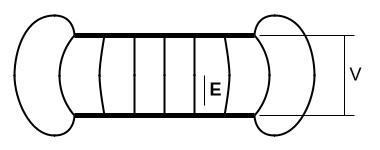
\includegraphics[width=200pt]{svg/capacitor.pdf}
    %\includegraphics[bb=0mm 0mm 100.0mm 170.0mm, scale=0.35, type=pdf]{img/problem7.pdf}
\end{figure}
\end{frame}


\end{document}

